\chapter{Evaluation}
\label{chapter:Evaluation}

The focus of the evaluation will be on the different runtimes of the various possible backends. These will be evaluated by running varouis prepared Jayvee models on one underlying dataset.

\section{Data source}
\label{section:data_source}

\subsection{Requirements}
%TODO: why not functional vs non-functional
\label{subsection:data_source_requirements}
\begin{enumerate}
	\item The dataset has to be available in a csv format, because the interpreter can only create tables from csv data.
	\item The dataset must contain a column with a numeric data type.
	\item The dataset should be a minimum of $800\text{MB}$, to make the backend's differences in speed visible.
	\item The dataset should not be larger than $3\text{GB}$, because open-datasets are usually not that big. %FIXME: citation needed +  everything.
	\item The dataset must have a licence conformant with the Open Definition. List here: \url{http://opendefinition.org/licenses/} % TODO: explanation.
\end{enumerate}


\subsection{Chosen Dataset}
The chosen dataset is called "Brewery Operations and Market Analysis" and not based on any real wold data, but rather generated by a python script \autocite{dataset}.

\subsubsection{Fulfilled requirements}
- license is \ac{ODbL} so one is fulfilled
- fits within the maximum and minimum filesize
- contains columns with integer and columns with floating point numbers.
- the dataset is contained in a single csv file.

\subsubsection{Biases}
- dataset does not benefit any backend specifically

\section{Parameters}
\label{section:parameters}
- what optimizations to use:
- typescript(none),
- pl: polars tables, columns and block executor, includes transforms but not RustSQLiteLoaderExecutor
- plob: pl + LocalFileToTableInterpreter
- plrs: pl + RustSQLiteLoaderExecutor
- plobrs(plob + plrs)
- how many transformations: none, some, many
- how many lines of data should be processed: $6$ steps $56250$, $112500$, $225000$, $4500000$, $900000$ ,$1800000$
- how often each configuration should be run: 100 times


\section{evaluation tool}
- cli allows to specify one or multiple values for the parameters.
- no value for a parameter means all possible values are used
- create configuration for every possible combination of linecount, transformation amount and activated optimizations (6 * 3 * 5) = 90 configs.
- run each config 100 times, save duration
- calculate average and standard deviation per config

- the output databases are checked for equality using sqldiff

\section{evaluation models}
- six models exist:
- 1-3: csv to table is done the usual way, then  *3 for no transforms, some transforms, and many transforms.
- 4-5: use the new block, then  *3 for no transforms, some transforms, and many transforms.
- no transforms: self explanatory
- some transforms:
- add column with ones
- sum "bitterness + volumes produced" into new col
-  "pH\_level" times 10 000, replace
- square root of total sales, new column

\subsection{run configs}
- use `head` to create csv files with the appropriate linecount from the downloaded csv
- pick the fitting model based on the config
- the models get the path of the source file and the path of the destination from a command line parameter (-e)



\section{Max file size}
\subsubsection{ts}
- ts can do 1 900 000 lines (475 mb), can't do 2 000 000 lines(500mb)
- sqlite loader fails with invalid string lenght error when inserting the rows
- sqlite loader might surpass the maximum string length limit when creating the insert values sql statement

\subsubsection{pl}
- works at 1 800 000 lines (450 mb)
- fails at 1 900 000 lines with heap out of memory, during inserting the rows into the db
- still has typescript implementation of the sqlite loader -> node restrictions apply.

\subsubsection{plob}
- works at 1 900 000 lines but nut 2 000 000 lines (invalid string lenght error)
- also does sql statement generation in node

\subsubsection{plrs}
- can do the 2 000 000 lines the node-sqlite limitations don't apply, it uses the rust stuff
- can't do 2 100 000 lines (525MB) because error: Cannot create a string longer than 0x1fffffe8 (536 870 888) characters.

\subsubsection{plobrs}
- only plobrs can process the full $10_000_000$ (2.5gb) lines.

\section{the numbers}
%TODO: pie chart of supported transfrorms
%TODO: stuff that is not supported by jayvee

\begin{figure}
	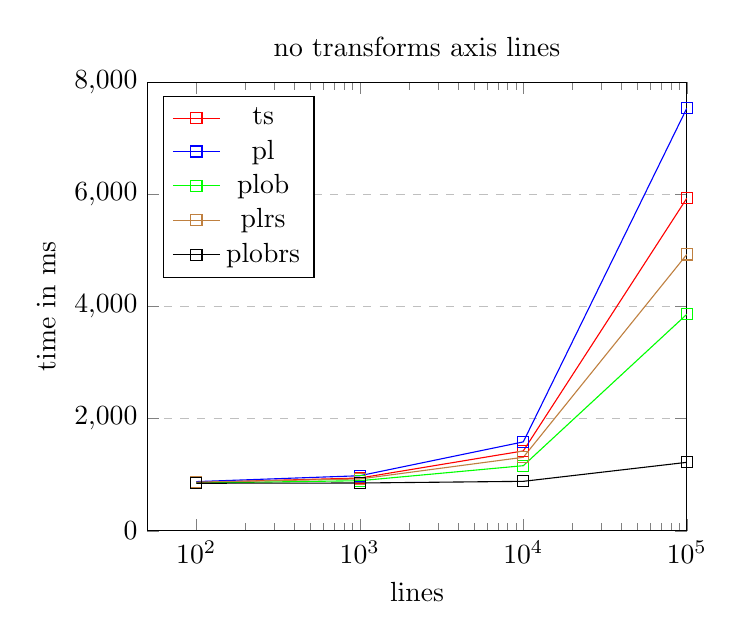
\begin{tikzpicture}
		\begin{semilogxaxis}[
				title = {no transforms}
				axis lines = left,
				xlabel = {lines},
				ylabel = {time in ms},
				xmin=0, xmax=100000,
				ymin=0, ymax=8000,
				xtick={0,100,1000,10000,100000},
				% ytick={0,1000,2000,3000,4000,5000,6000},
				legend pos=north west,
				ymajorgrids=true,
				grid style=dashed,
			]
			\addplot[
				color = red,
				mark=square,
			]
			coordinates {
					(100,864)(1000,942)(10000,1426)(100000,5935)
				};
			\addplot[
				color=blue,
				mark=square,
			]
			coordinates {
					(100,878)(1000,983)(10000,1587)(100000,7541)
				};
			\addplot[
				color=green,
				mark=square,
			]
			coordinates {
					(100,853)(1000,894)(10000,1162)(100000,3864)
				};
			\addplot[
				color=brown,
				mark=square,
			]
			coordinates {
					(100,869)(1000,925)(10000,1312)(100000,4932)
				};
			\addplot[
				% color=orange,
				mark=square,
			]
			coordinates {
					(100,849)(1000,853)(10000,883)(100000,1222)
				};
			\legend{ts,pl,plob,plrs,plobrs}
		\end{semilogxaxis}
	\end{tikzpicture}
	\caption{plot no transforms}\label{fig:plot}
\end{figure}

